Firstly, we looked at the correlation between length and frequency graphically by plotting 6 languages with length as a function of word frequency in \cref{plot1}.

\begin{figure}[h]
\centering
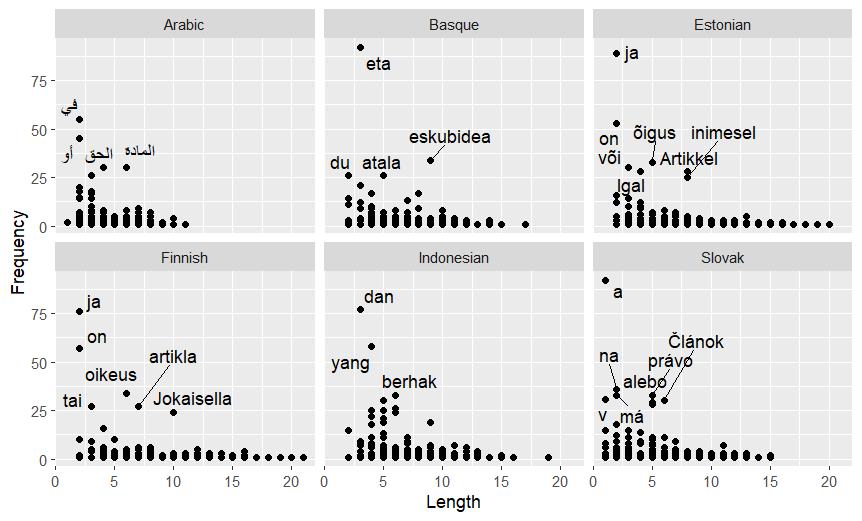
\includegraphics[width=\textwidth]{images/plot1.png}
\caption{Length as a function of word frequency for Arabic, Basque, Estonian, Finish, Indonesian and Slovak.}
\label{plot1}
\end{figure}

\newpage
Also, in order to statistically check for the correlation, we ran the  Kendall tau correlation test on the data for all the 20 selected languages and obtained the value of tau and p-value for each language. We also ran a Holm-Bonferroni correction on the p-values. This data is summarized in \cref{table1}.

\begin{table}[]
\begin{tabular}{lllllll}
Language   & Family         & Tokens & Types & Tau     & p-value  & C. p-value \\ \hline
Arabic     & Austronesian   & 1318   & 725   & -0.203  & 1.13e-10 & 1.02e-09   \\
Basque     & N/D            & 1236   & 652   & -0.242  & 5.06e-14 & 8.09e-13   \\
Bulgarian  & Indo-European  & 2273   & 653   & -0.229  & 3.46e-13 & 4.5e-12    \\
Chinese    & Sino-Tibetan   & 2693   & 532   & -0.189  & 8.07e-07 & 4.84e-06   \\
Estonian   & Uralic         & 1250   & 654   & -0.237  & 1.56e-13 & 2.19e-12   \\
Finnish    & Uralic         & 1113   & 672   & -0.208  & 8.17e-11 & 8.17e-10   \\
German     & Indo-European  & 1330   & 545   & -0.303  & 1.3e-18  & 2.59e-17   \\
Indonesian & Austronesian   & 1302   & 488   & -0.159  & 1.11e-05 & 3.33e-05   \\
Irish      & Indo-European  & 1640   & 598   & -0.268  & 5.16e-16 & 9.79e-15   \\
Japanese   & Japonic        & 2325   & 517   & -0.101  & 1e-02    & 2.01e-02   \\
Kannada    & Dravian        & 401    & 304   & -0.0787 & 9.81e-02 & 9.81e-02   \\
Korean     & Koreanic       & 996    & 557   & -0.176  & 2.84e-06 & 1.14e-05   \\
Malay      & Astronesian    & 1288   & 462   & -0.177  & 2.16e-06 & 1.08e-05   \\
Polish     & Indo-European  & 1334   & 655   & -0.238  & 7.46e-14 & 1.12e-12   \\
Setswana   & Atlantic-Congo & 1735   & 459   & -0.298  & 1e-15    & 1.8e-14    \\
Slovak     & Indo-European  & 1444   & 726   & -0.235  & 1.53e-14 & 2.6e-13    \\
Spanish    & Indo-European  & 1559   & 509   & -0.254  & 8.68e-13 & 1.04e-11   \\
Tagalog    & Afro-Asiatic   & 1509   & 453   & -0.214  & 1.25e-08 & 9.96e-08   \\
Turkish    & Turkic         & 1310   & 696   & -0.208  & 2.7e-11  & 2.97e-10   \\
Yoruba     & Atlantic-Congo & 1437   & 385   & -0.221  & 4.39e-08 & 3.07e-07  
\end{tabular}
\caption{Table displaying family, tokens, types, tau, p-value and corrected p-value for the 20 selected languages.}
\label{table1}
\end{table}

\newpage
After the statistical tests, we also computed other metrics which can be useful to identify patterns and better understand our results. We calculated the mean word length ($L$), the minimum baseline ($L_{min}$) and the random baseline ($L_r$). After obtaining the previous values, we also computed the degree of optimality ($\eta$) and the optimality score ($\Omega$). We summarized this data in \cref{table2}.

\begin{table}[]
\begin{tabular}{lllllll}
Language   & Family         & $L_{min}$ & $L$    & $L_r$   & $\eta$     & $\Omega$     \\ \hline
Arabic     & Austronesian   & 4.06 & 4.67 & 5.42 & 0.87  & 0.553 \\
Basque     & N/D            & 5.77 & 6.75 & 7.99 & 0.855 & 0.558 \\
Bulgarian  & Indo-European  & 2.83 & 3.57 & 6.17 & 0.791 & 0.777 \\
Chinese    & Sino-Tibetan   & 1.01 & 1.01 & 1.05 & 1     & 1     \\
Estonian   & Uralic         & 5.83 & 6.7  & 8.43 & 0.869 & 0.664 \\
Finnish    & Uralic         & 6.83 & 7.68 & 9.3  & 0.889 & 0.656 \\
German     & Indo-European  & 5.17 & 6.29 & 8.5  & 0.822 & 0.665 \\
Indonesian & Austronesian   & 5.08 & 6.47 & 7.75 & 0.785 & 0.48  \\
Irish      & Indo-European  & 3.81 & 4.87 & 6.85 & 0.782 & 0.651 \\
Japanese   & Japonic        & 1.29 & 1.62 & 1.94 & 0.797 & 0.493 \\
Kannada    & Dravian        & 6.93 & 7.8  & 8.33 & 0.888 & 0.375 \\
Korean     & Koreanic       & 2.4  & 2.89 & 3.24 & 0.829 & 0.413 \\
Malay      & Astronesian    & 5.13 & 6.49 & 7.69 & 0.791 & 0.47  \\
Polish     & Indo-European  & 5.18 & 6.26 & 8.04 & 0.828 & 0.624 \\
Setswana   & Atlantic-Congo & 3.46 & 4.59 & 7.31 & 0.755 & 0.707 \\
Slovak     & Indo-European  & 4.67 & 5.65 & 7.23 & 0.827 & 0.617 \\
Spanish    & Indo-European  & 4.02 & 5.18 & 7.6  & 0.776 & 0.675 \\
Tagalog    & Afro-Asiatic   & 4.23 & 5.42 & 7.98 & 0.78  & 0.682 \\
Turkish    & Turkic         & 5.5  & 6.4  & 7.63 & 0.86  & 0.578 \\
Yoruba     & Atlantic-Congo & 2.73 & 4.03 & 4.93 & 0.677 & 0.408
\end{tabular}
\caption{Table displaying family, tokens, types, mean word length ($L$), the minimum baseline ($L_{min}$), the random baseline ($L_r$), the degree of optimality ($\eta$) and the optimality score ($\Omega$) for the 20 selected languages.}
\label{table2}
\end{table}

\newpage
With the data represented in \cref{table2}, we created a plot which shows $L_r$ as function of $L$ in order to visualize it in \cref{plot2}. We also included $L_{min}$ encoded as the size of the dots to add a third dimension to the data and visualize $L$, $L_r$ and $L_{min}$ at the same time.

\begin{figure}[h]
\centering
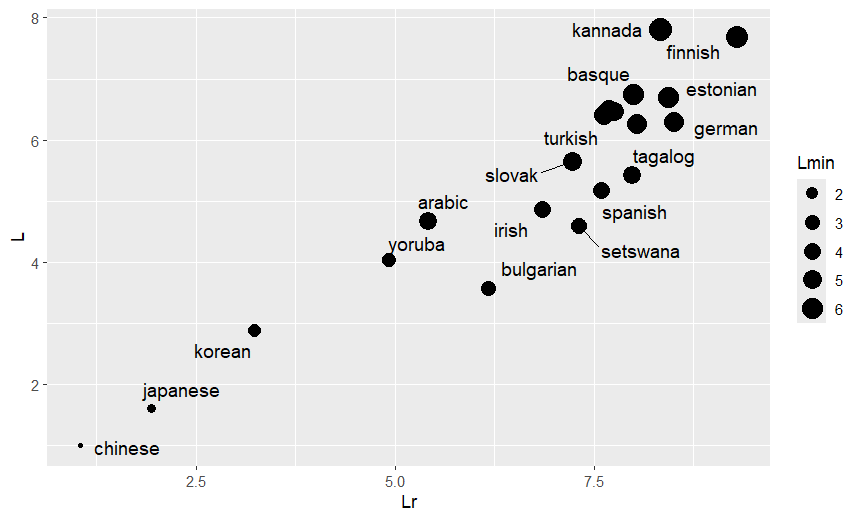
\includegraphics[width=\textwidth]{images/plot2.png}
\caption{$L_r$ as function of $L$ with $L_{min}$ encoded as dots size for the 20 selected languages.}
\label{plot2}
\end{figure}
